\problemname{Formula Flatland}

\illustration{0.32}{TurnTen}{Part of a street circuit. Photo by Ronnie Boone, \href{https://en.wikipedia.org/wiki/File:TurnTen.jpg}{wikipedia}\vspace{-0.5cm}}
Flatland is happy to announce that this year -- for the first time ever -- the Formula One comes to Flatland to arrange the Grand Prix of Flatland.
As with many other cities, Flatland is not able to build a dedicated circuit for the race.
Therefore, Flatland decided to close off some of its normal streets and crossings to form a circuit.
After your excellent work as an organizer of last year's \emph{Flatland Olympics}, you were hired to find a suitable circuit.
Since closed off streets are annoying to the people who live there, you would like to minimize the number of crossings that need to be closed off for the race.

\begin{figure}[h]
	\centering
	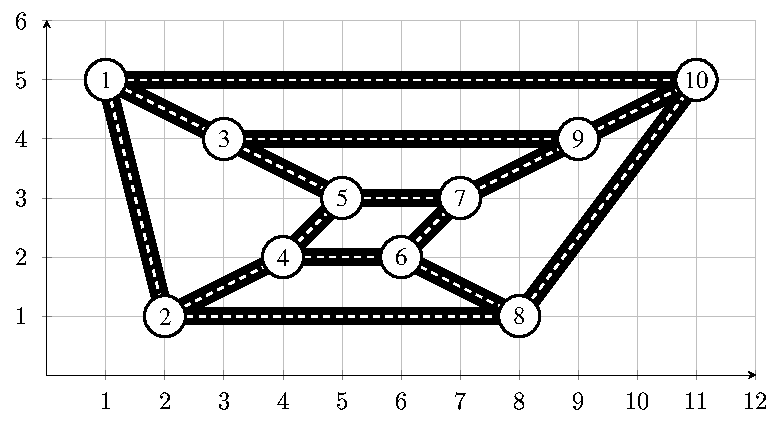
\includegraphics[width=0.7\textwidth]{sample1}
	\caption{Visualization of the first sample.
		One possible optimal circuit would be: $(4,5,7,6)$.}
\end{figure}

Your job only consists of selecting some road segments which form a circle but are connected by as few crossings as possible.
Note that even though all roads in Flatland are bidirectional, they can only be used in one direction during the race for safety reasons.

\begin{Input}
	The input consists of:
	\begin{itemize}
		\item One line with two integers $n$ and $m$ ($4\leq n \leq10^5\text{ and }5\leq m\leq3\cdot10^5$), the number of crossings and the number of road segments in Flatland.
		\item $n$ lines, each with two integers $x$ and $y$ ($0\leq x,y\leq10^9$), the $i$th line describes the position of the $i$th crossing on a map of Flatland.
		No two crossings are at the same position.
	\item $m$ lines, each with two integers $a$ and $b$ ($1\leq a,b\leq n\text{ and }a\neq b$), describing that the $a$th and $b$th crossing are connected by a road segment.
		Two crossings are connected by at most one road segment.
	\end{itemize}
	It is guaranteed that two road segments only intersect in a crossing they both start or end at.
	Further, it is guaranteed that each crossing on the map corresponds to an actual crossing in the sense that at least three road segments intersect.
\end{Input}

\begin{Output}
	Output a single integer, the minimum number of crossings the racetrack must contain.
\end{Output}

